%%%%%% CMB-S4 Simulations and Data Analysis Chapter, Sky Modeling Section  %%%%%%%%%%%%%%%%

%\section{Sky Modeling}
%
%Key challenges: 
%\begin{itemize} 
%\item reliability of models based on noisy, bandpassed, beam-convolved observations, including Planck
%\item self-consistency of CMB secondaries and extra-Galactic foregrounds
%\item usability/software engineering
%\end{itemize} 
%
%%%%%% CMB-S4 Simulations and Data Analysis Chapter, Sky Modeling Section  %%%%%%%%%%%%%%%%

\section{Sky Modeling}
\label{sec:skymodel}

The capability of CMB-S4 to address its science program crucially depends on the possibility to separate the signals of interest from astrophysical emission originating from various astrophysical processes, and on the accuracy of the characterization of foreground residuals after such cleaning is performed. 

The polarized CMB is mostly contaminated by diffuse emission from the interstellar medium of our own Milky Way. Both synchrotron and thermal dust are polarized---up to the level of tens of percents, depending on the observed region). Their integrated emission dominates over both the CMB E-modes and the CMB B-modes on large angular scales, and cannot be safely neglected at scales where B-modes from gravitational lensing dominate without robust analyses of their impact on lensing science. Other components, such as spinning dust, free-free emission, emission of molecular lines such as CO, could in principle be polarized at a lower level, of order 1-2 per cent or less, but measurements or upper limits are scarce, and not sufficient at this stage for robust predictions of the polarized amplitude of their emission over large patches of sky. For science on smaller angular scales, the presence of polarized extragalactic radio and infrared sources constitutes an additional source of contamination, which must be removed with a combination of masking or subtracting individual sources, and modeling residuals at the power-spectrum level.

%Massive galaxy clusters are easily detected in atmospheric windows below 217 GHz (and in particular around 150 GHz) as decrements in high angular resolution maps of total sky emission fluctuations. The detection of low-mass, distant galaxy clusters, however, will suffer from confusion with fluctuations of the CIB emission (which can be locally positive or negative), and from contamination by radio and infrared sources in the cluster halos. Accurate determination of the clusters' profiles, of their integrated Compton parameter $Y$ that serves as a mass-proxy for cosmological constraints, and of cluster peculiar velocities along the line of sight via the kinematic SZ effect, will require sufficient frequency coverage at high angular resolution (of order 1-2$^\prime$) to separate the various SZ components (thermal SZ, relativistic corrections, and kinematic SZ) as well as sources of astrophysical confusion. In particular, it is plausible that high angular resolution observations of the positive side of the SZ effect (at frequencies above 217 GHz) will be required to fully exploit the sensitivity of CMB-S4 for galaxy cluster science.

Estimating more precisely the impact of foreground emission on the main science targets of CMB-S4 will require realistic simulations of the sky emission that can be used to test the effectiveness of component separation techniques and to assess any degradation of the error bars or possible biases due to residual foreground contamination. 
Figure~\ref{fig:skymodel-in-pipeline} locates this modelling within the larger CMB simulation and data analysis pipeline.

\begin{figure}[htbp]
\centering
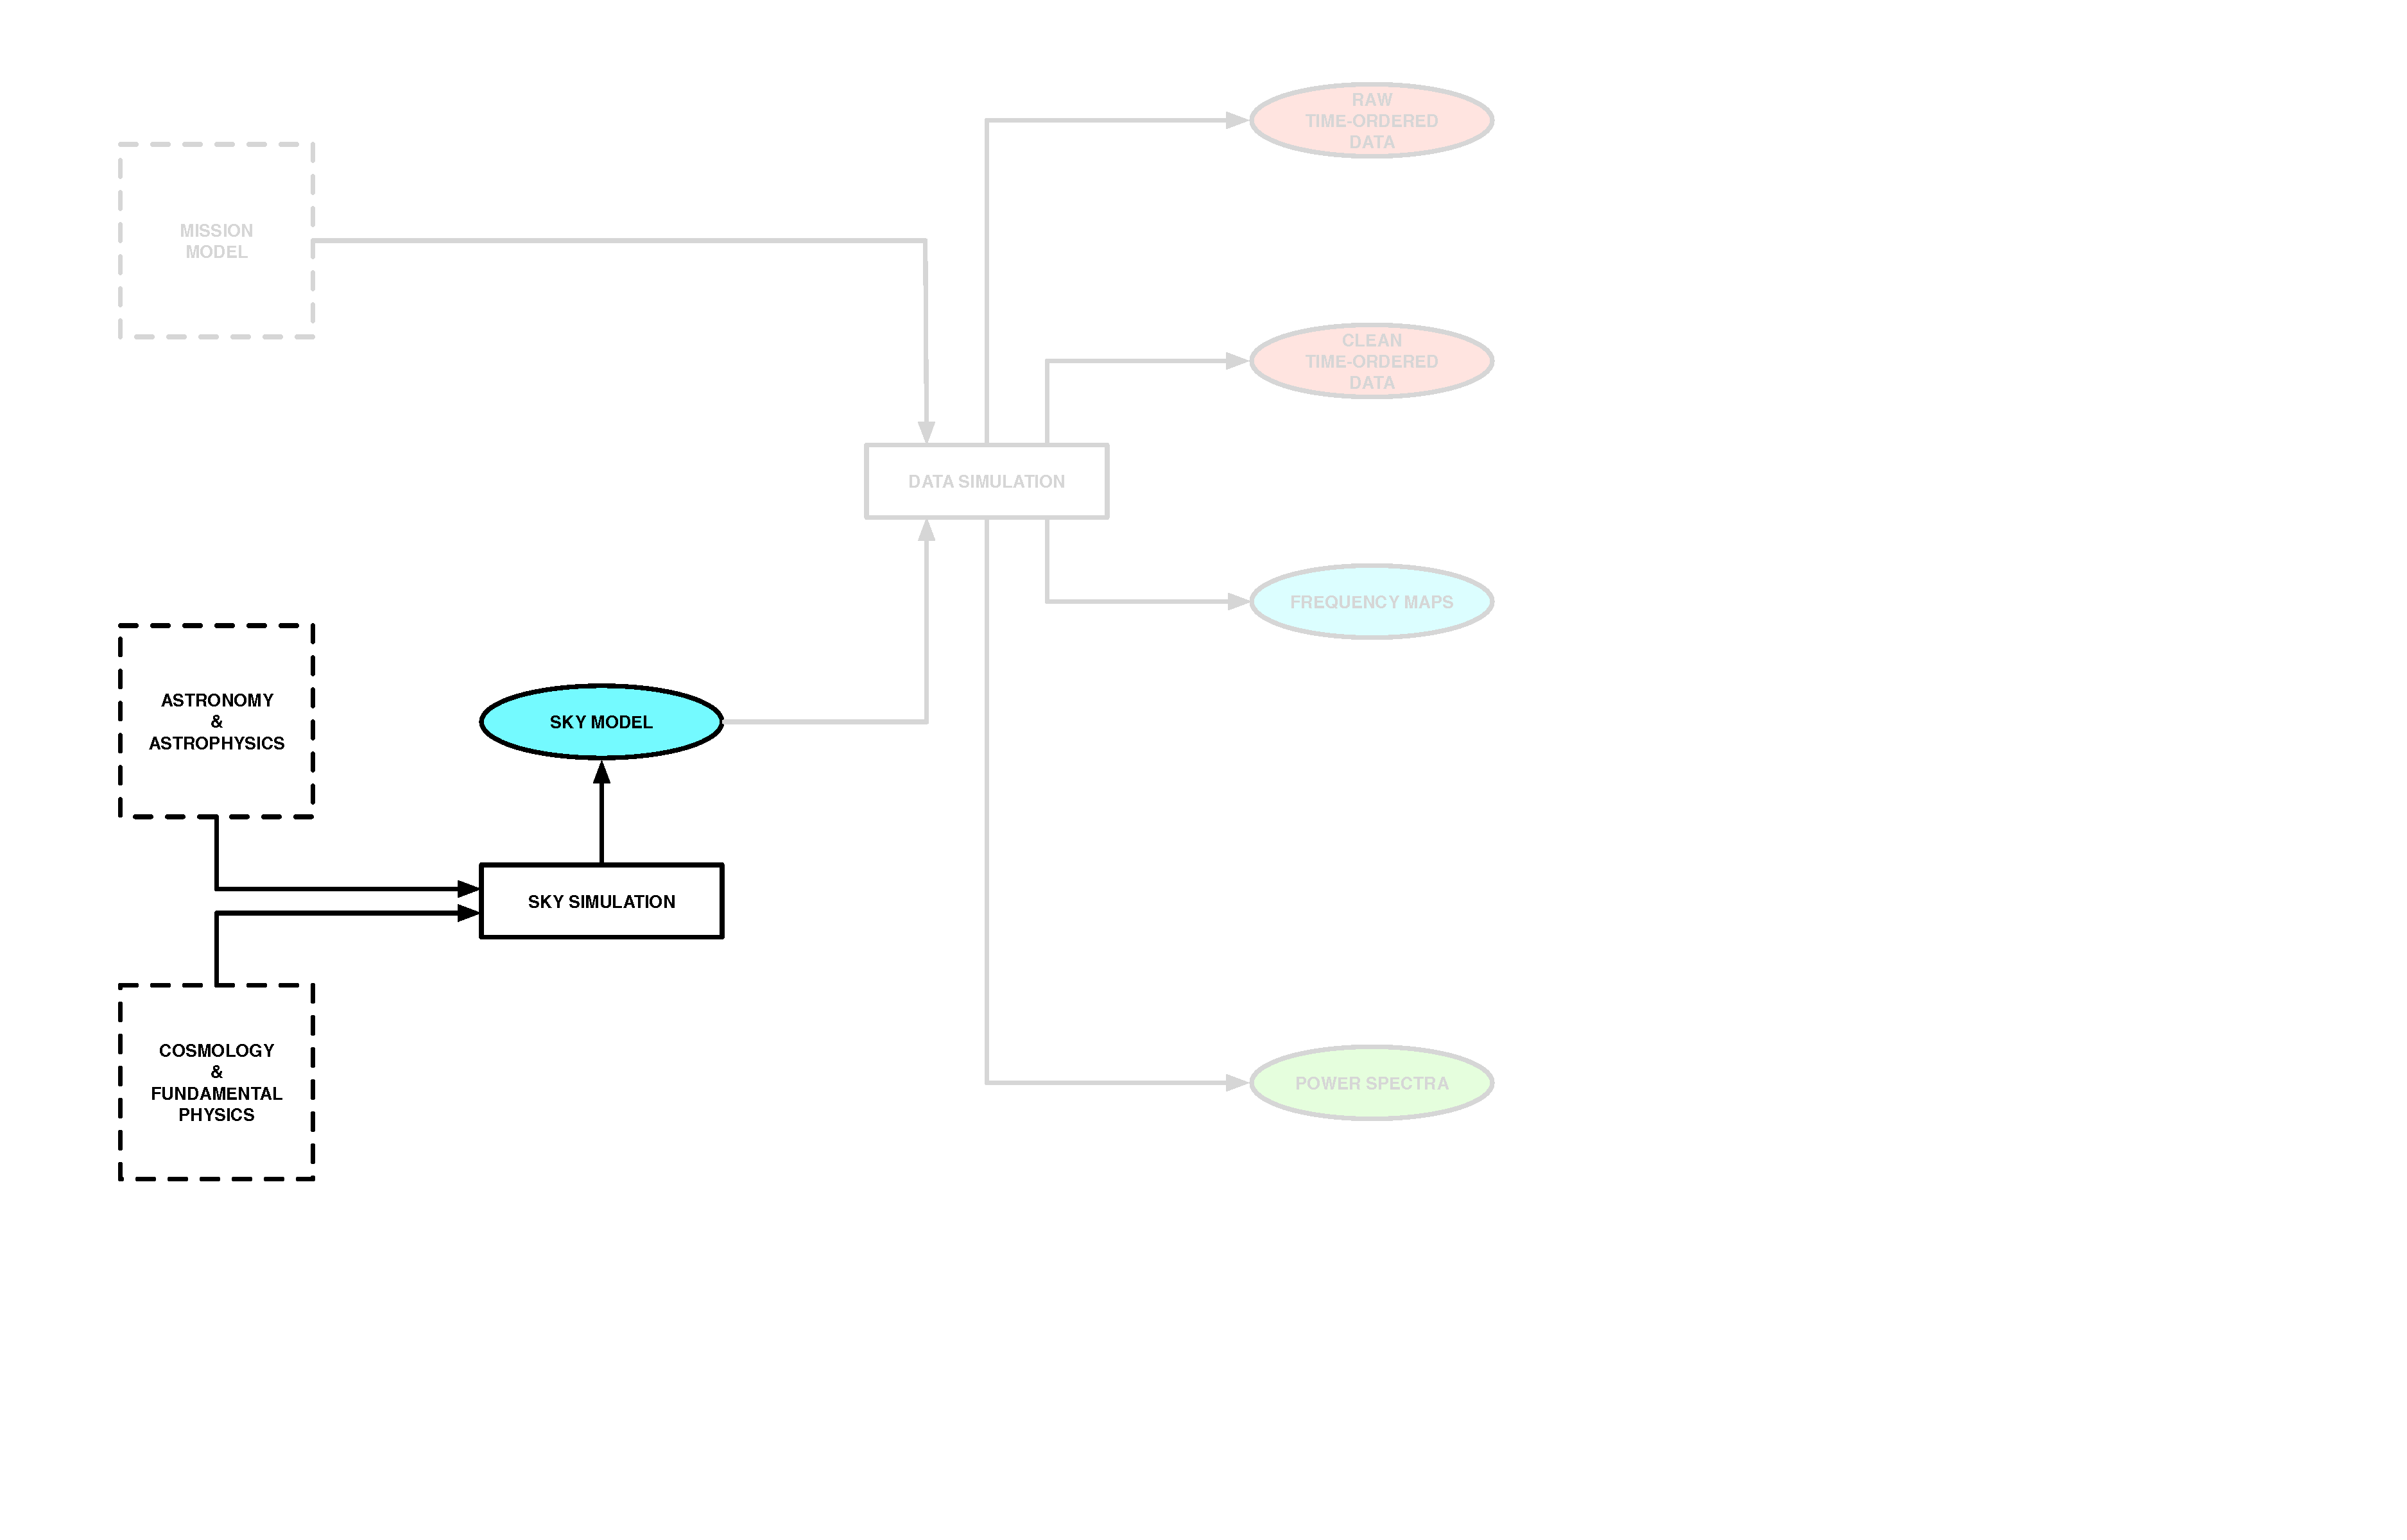
\includegraphics[width=0.5\textwidth]{Analysis/sm}
\caption{The sky modelling subset of the CMB simulation pipeline. The full simulation pipeline is shown in Figure~\ref{fig_sim}.}
\label{fig:skymodel-in-pipeline}
\end{figure}


The sky emission is naturally modeled as the sum of emission from different sources. These sources may identified by their emission process (e.g. Galactic synchrotron, due to electrons spiralling in the Galactic magnetic field), or by their place of origin (e.g. emission of a particular extragalactic source). These emissions, as a function of sky pixel and frequency, must then be band-integrated and beam-integrated to produce total emission maps as observed by the instrument. 
%We decompose this simulation pipeline into two main steps: the multicomponent model of sky emission, which does not depend on the instrument, and the integration of this emission in the instrumental response.
This latter part of the simulation pipeline is treated in Section \ref{sec_datasim}; we concentrate in this section on the sky model.

A sky model is useful only as far as it captures adequately the characteristics of real sources of sky emission that play an essential role in the performance of cleaning techniques and on the amplitude and statistical properties of residual contamination after such cleaning is performed. The key characteristics of sky emission for foreground cleaning are:
\begin{itemize}
\item The coherence and decoherence of diffuse emission across observed frequencies, which is key to identifying foreground emission in the form of patterns that scale with an emission law different from that of the CMB;
\item The existence or not of a simple parametric emission law for each component emission, such as power laws (for synchrotron) or modified blackbody emission (for dust components);
\item The absolute level of foreground emission (in particular for those components that do not scale simply as a function of frequency, such as the superposition of many individual sources with a specific emission law each);
\item Whether or not emissions for which the level of polarization is unknown or unclear (including possible surprises) are above the sensitivity objectives of CMB-S4, or can be safely neglected;
\item The self-consistency of extragalactic emission (in particular CIB and SZ clusters) and CMB lensing. In particular, CIB as observed by Planck and by future instruments can be used to generate a proxy for the lensing potential, which can be used to partially de-lens the CMB B-modes.
\end{itemize} 


The key challenges for constructing a sky model are hence:
\begin{itemize} 
\item The reliability of models based on observations at angular resolution lower than that of CMB-S4, integrated in broad frequency bands, and with a sensitivity limit at least an order of magnitude worse than what will be achieved with CMB-S4; the complexity of sky emission below current sensitivity limits must be extrapolated on the basis of existing knowledge and theoretical models, taking into account past experience when orders of magnitude in sensitivity were gained;
\item The self-consistency of CMB secondary anisotropies (lensing, SZ emission from hot intra-cluster gaz and filaments, late ISW) and extra-Galactic foregrounds (CIB, radio and infrared sources) is crucial to both de-lensing, and to extragalactic science; generating reliable models over the entire Hubble volume is challenging, the evaluation of errors of such models even more so;
\item The practical usability of the model (software engineering aspects for generating many simulations).
\end{itemize} 


%\subsection{The sky modeling pipeline}
%
%The emission of the sky will be modeled as the sum of emission of different components, identified either by their emission process (e.g. Galactic synchrotron, due to electrons spiralling in the Galactic magnetic field), or by their region of origin (e.g. emission of a particular extragalactic source). These emissions, as a function of sky pixel and frequency, must then be band-integrated and beam-integrated to produce total emission maps as observed by the instrument. 
%%We decompose this simulation pipeline into two main steps: the multicomponent model of sky emission, which does not depend on the instrument, and the integration of this emission in the instrumental response.
%This latter part of the simulation pipeline is treated in Section \ref{sec_datasim}; we concentrate in this section on the sky model.

%\subsubsection{The multi-component sky model}

%\subsubsection{Sky emission observations}

\subsection{The Galactic interstellar medium}

Strong evidence exists for variability of the physical properties of the interstellar medium of the Milky Way as a function of the line of sight. This variability implies that the properties vary across different regions of the Milky Way, with the total ISM emission in each line of sight being a superposition of emission from various regions. Even assuming that each such region has a simple parameteric emission law, such as a power law or a modified blackbody, the superposition of such emission cannot be modeled with a single simple emission law. Modeling the Galactic ISM for future sensitive surveys such as CMB-S4 requires  modeling  this complexity at the appropriate level. It seems reasonable to use a multi-layer approach, in which each ISM component is modeled as a superposition of several layers, with a simple (although pixel-dependent and polarization dependent) emission law for each such layer.

\subsubsection{Synchrotron}

The baseline Galactic synchrotron model we use here has a power law scaling with a modestly spatially varying spectral index.  The emission templates are the Haslam 408 MHz data reprocessed by \cite{remazeilles16}, 
%MNRAS 451, 4311,
and the WMAP 7-year 23 GHz Q/U maps \cite{jarosik11}
% ApJS, 192, 14J) 
smoothed to 3 degree FWHM and with smaller scales added using the PSM code \cite{delabrouille13}
% et al. A&A 553, A96, 2013). 
The spectral index map is derived using a combination of the Haslam 
408 MHz data \cite{haslam81} and WMAP 23 GHz 7-year data \cite{miville-deschenes08}
% M.-A. et al., 2008, A&A, 490, 1093). 
The same scaling is used for intensity and polarization.  This is the same prescription as used in the Planck Sky Model's v1.7.8 `power law' option, but with the Haslam map updated to the version in \cite{remazeilles16}.

Extensions to this model that we are exploring include a curved power 
law model with a single isotropic curvature index, and a polarization spectral index that steepens with Galactic latitude by $\delta \beta \sim 0.2$ from low to high latitude, as this is currently consistent with WMAP and Planck data. 

\subsubsection{Thermal dust}
The baseline model we consider has thermal dust modelled as a single component modified  blackbody. We use dust templates for emission at 545 GHz in intensity and 
 353 GHz in polarization from the Planck-2015 analysis, and scale these to different  frequencies with a modified black-body spectrum using the spatially varying dust temperature and emissivity obtained from the Planck data using the Commander code \cite{planck15-10}. This therefore assumes the same spectral index for  polarization as for intensity.  These templates are smoothed to degree scale.

Variations on this model that appear consistent with current data are a more strongly varying emissivity, e.g. up to $\sigma \sim 0.2$ dispersion on degree scales,  in addition to different prescriptions for small-scale behaviour that account for turbulence in the magnetic field. A two (or more) component model for the dust, composed of the spatially varying sum of silicon and carbonaceous dust, each with a different emissivity, is also physically motivated.

\subsubsection{Spinning dust}
Spinning dust, or anomalous microwave emission, is nominally unpolarized. However, a fractional polarization of a few percent is physically possible and not excluded by current data. We construct a possible model for this polarization using the intensity templates for spinning dust from the Planck-2015 Commander fits
\cite{planck15-10}, combined with the thermal dust polarization angles and an overall polarization fraction.

%\subsubsection{Free-free}

%\subsubsection{Atomic and molecular lines}

\subsubsection{Other components}
Other contributions to the intensity and polarization of the Milky Way at \cmbexp\ frequencies, such as 
free-free emission and molecular line emission, are not expected to be at the same amplitude and degree
of polarization as the components treated individually above. However, the full sky model will need to include
these components in at least the most pessimistic scenarios, unless further data is obtained that 
conclusively demonstrates they can be fully neglected.

\subsection{CMB Secondary Anisotropies and Extragalactic Sources}

The key goal for the extragalactic sky models of CMB-S4 is to provide fast and self-consistent simulations of CMB secondary anisotropies and extragalactic sources. These models will allow us to make more realistic forecasts. In our cosmological analyses they will allow us to Monte Carlo over the underlying astrophysical uncertainties of these secondaries and sources. Our plan to meet these challenges is modular and can be broken down as follows: 

\begin{itemize}
\item We will use full hydrodynamical simulations of cosmological volume as the basis to parametrically model the complicated {\it gastrophysical} processes associated with extragalactic foregrounds.
\item As the backbone of our model we will require fast simulations of growth of structure that generate halo catalogs for a large set of cosmological parameters.
\item To have self-consistent maps we will have a flexible pipeline that generates simulated all sky maps which applies the parametric models from the hydrodynamical simulations to our backbone large-scale structure simulations and halo catalogs.
\end{itemize}

Hydrodynamical simulations of cosmological volumes are currently available which we can already use to model extragalactic foregrounds. These simulations will be used for the development and testing phases of the simulation pipeline. However, they are limited in their size and sub-grid modeling accuracy, and thus will not meet our accuracy requirements of CMB-S4. We will develop new full hydrodynamical simulations of cosmological volumes that include a variety of physical processes. An essential requirement of these simulations will be to capture growth and evolution of galaxies to cluster-size halos throughout cosmic time at a sufficient spatial resolution. Hydrodynamic simulations of this size and scale are already computationally feasible, the challenges will be the appropriate modeling of radiative cooling, star formation, and feedback processes in order to capture the global stellar and gas contents of these halos.

There are many different approaches already developed to provide us with the underlying large-scale structure simulations that will we build our extragalactic model upon. They vary in speed which tend to inversely scale with accuracy. A benefit of our modular and flexible approach is that we do not need to limit ourselves to one approach. In fact we will compare the various approaches to see how they bias our answers. It is in these simulations where we will vary cosmological parameters assuming that they only affect the growth of structure and not the {\it gastrophysical} properties of extragalactic foregrounds.

Our final product will be all sky maps. They will be in HEALPIX format to seamlessly interface with galactic and CMB simulated maps. The map products will include:

\begin{itemize}
\item Optical galaxies that correspond to the various overlapping surveys including LSST.
\item Radio and dusty star-forming galaxy point sources.
\item Unresolved CIB.
\item Projected density maps (both total and gas) of the large-scale structure.
\item Thermal and kinetic SZ maps.
\end{itemize}

\noindent We will explore the parameter space for each of the maps listed above and provide a sufficient number of realizations that we can marginalize over the many model uncertainties. For example, the lensing field can be constructed through a proper ray-tracing method from the projected density maps or via the Born approximation. Our self-consistent extragalactic sky model allows us to test various sources of contamination and systematic biases in our estimators. Additionally, any cross-correlation analyses can easily be checked and evaluated using these maps. {\bf All the simulation products we create will become public.}

%\bibliography{cmbs4}

%%
%% Populate the .bib file with entries from SPIRES Bibtex (preferred)
%% or ADS Bibtex (if no SPIRES entry).
%%  SPIRES will also supply the CITATION line information; please include it.
%%


